\documentclass[noframe,oneside]{ncuthesisCJK}
\usepackage{makeidx}             % for index
\usepackage{layout}
\usepackage[]{todonotes}

\usepackage{cite}

\usepackage{graphicx}
\usepackage{amsmath}
\usepackage{amssymb}
\usepackage{amsfonts}
\usepackage{epsfig}
\usepackage{subcaption}
\usepackage{indentfirst}
\usepackage{color}
%\usepackage{txfonts}
%%%%%%%%%%
\usepackage{esvect}
\usepackage{epstopdf}

%\usepackage{algorithmic}
\usepackage[normalem]{ulem}
\usepackage{mathtools}
%\usepackage{txfonts}
\captionsetup{compatibility=false}
\graphicspath{{./figures/}}
%\newtheorem{definition}{Definition}
%\newtheorem{lemma}{Lemma}
\makeatletter
\renewcommand*{\@opargbegintheorem}[3]{\trivlist
      \item[\hskip \labelsep{\bfseries #1\ #2}] \textbf{(#3)}\ \itshape}
\makeatother
\usepackage{graphicx}
\usepackage{CJKutf8}
\usepackage{amsmath}
\usepackage{amssymb}
\usepackage{amsthm}
\usepackage{amsfonts}
\usepackage{epsfig}
\usepackage{subcaption}
\usepackage{indentfirst}
\usepackage{xcolor}
\usepackage{esvect}
\usepackage{epstopdf}
\usepackage[normalem]{ulem}
\usepackage{lipsum}
\usepackage{subcaption}
%\usepackage{gensymb}

\usepackage{multirow}
\usepackage{float}
\usepackage[ruled,lined]{algorithm2e}
\usepackage{algcompatible}

\usepackage[normalem]{ulem}
\usepackage{tabularx}
\usepackage{float}
\usepackage{caption,subcaption}
\captionsetup{compatibility=false}
\SetKwInOut{Parameter}{Parameters}
\SetKwInOut{INIT}{Initialization}
\usepackage{makecell}
\usepackage{afterpage}
\usepackage{booktabs}


\dept{數學研究所}
\degree{碩士}
\title{Multi-robot Search in 3D Environments using Submodularity with Matroid Intersection Constraints}
\subtitle{}
\author{李晏碩}
\authoren{Yan-Shuo, Li}
\mprof{曾國師}
\mprofen{Kuo-Shih, Tseng}
\sprof{}
\degreedate{中~華~民~國~一百一十三~年~六~月}
\copyyear{2024}
\def\XeLaTeX{Xe\LaTeX}   % Only in CJK
\input{mypreamble}             % 自訂巨集多 收起來
                                            % 自訂巨集少 直接寫出

%\includeonly{chapter2}      % 單獨編譯此檔
\makeindex                           % 告訴\LaTeX要做索引
\begin{document}                 % 宣告結束   本文開始
\begin{CJK}{UTF8}{bkai}   %----------------------
\CJKhorz
\fontsize{14pt}{20pt}\selectfont % 可調間距以便閱讀%
\pagenumbering{alph}               % to cheat latex
\maketitle                       % 論文封面
\setboolean{printcopyright}{true}
\maketitle                       % 書名面
\cleardoublepage
\addtocontents{toc}{~\hfill\textbf{Page}\par}
%\includepdf[pages=-,scale=0.9]{4.pdf}
%\includepdf[pages=-,scale=0.9]{3.pdf}
\includepdf[pages=-,scale=0.9]{1.pdf} % 插入其他表格
\includepdf[pages=-,scale=0.9]{2.pdf} % 插入其他表格

\pagenumbering{roman}          % 羅馬數字編頁
\title{Multi-robot Search in 3D Environments using Submodularity with Matroid Intersection Constraints}
\begin{abstractcn}
%
\index{ncuthesis 環境!abstractcn}

{\bf \sf 關鍵字:} 次模性, 擬陣理論, 多機器人搜尋問題, 任務分配問題

\vspace{2em}

多機器人搜尋是一個具有挑戰性的問題,因為其涉及任務分配和覆蓋問題,而這些問題皆是NP-hard。
它可以重新定義為在擬陣限制下的覆蓋率最大化問題。
覆蓋率最大化問題可透過次模性來解決。
擬陣限制是由路徑限制和分群限制所組成。
此研究提出Multi-robot Search with Matroid constraints (MRSM)的方法,此方法達成$\frac{1}{3}\widetilde{OPT}$,其中 $\widetilde{OPT}$ 是基於生成樹結構下的近似最優性能。
實驗結果顯示,所提出MRSM方法在多機器人搜尋問題中優於其他演算法。
\end{abstractcn} 
\title{Multi-robot Search in 3D Environments using Submodularity with Matroid Intersection Constraints}
\begin{abstracten}
\index{ncuthesis 環境!abstracten}
{\bf \sf Keywords:} Submodularity, Matroid, Multi-robot search problem, Task allocation problem

\vspace{2em}

The multi-robot search problem is challenging since it involves task allocation and coverage problems, which are NP-hard.
This problem is reformulated as the maximal coverage problem subject to the intersection of matroid constraints.
The coverage problem is solved by utilizing its submodularity.
The intersection matroid is composed of a routing constraint and a clustering constraint.
The proposed algorithm, Multi-robot Search with Matroid constraints (MRSM), achieves $\frac{1}{3}\widetilde{OPT}$, where $\widetilde{OPT}$ is an approximately optimal performance under a spanning tree structure.
The experiment results show that the proposed approach outperforms state-of-the-art methods in multi-robot search problems.
\end{abstracten}

                 % 摘要
\begin{acknowledgements} \index{Acknowledgements}
\index{ncuthesis 環境!acknowledgements}

感謝指導教授、身邊的親朋好友和所有參與以及協助實驗的人員。
過程中,有大家的協助與鼓勵,是我莫大的榮幸!


%\begin{itemize}
%\end{itemize}
\end{acknowledgements}             % 謝誌
\cleardoublepage
\phantomsection\addcontentsline{toc}{chapter}{Contents}
\tableofcontents                 % toc
\cleardoublepage
\phantomsection\addcontentsline{toc}{chapter}{Figures}
%\renewcommand{\numberline}[1]{圖~#1\hspace*{1em}}%圖目錄
\listoffigures                   % lof
\cleardoublepage
%\renewcommand{\numberline}[1]{表~#1\hspace*{1em}}%表目錄
\phantomsection\addcontentsline{toc}{chapter}{Tables}
\listoftables                    % lot
\index{\LaTeX!\textbackslash phantomsection}
\index{\LaTeX!\textbackslash addcontentline}
\index{\LaTeX!\textbackslash hspace}
\include{symbol}                     % 符號說明     symbols 環境
\cleardoublepage

\pagenumbering{arabic}           % 阿拉伯數字編頁
                                 % \mainmatter
\chapter{Introduction}

The challenge of IPP is to find the optimal path that maximizes the information subject to budget constraints.
However, finding the optimal path is a NP-hard problem.
To solve these problems, some methods are proposed.
% Coverage-based planning is proposed to find a path that passes over all points of an area \cite{galceran2013survey}.
In \cite{popovic2017multiresolution}\cite{popovic2020informative}, the authors proposed an informative path planning framework in online settings with adaptivity requirements.
This approach enables agents to find a target based on the given constraints. However, these approaches cannot achieve the theoretical guarantees.



%{\color{olive}(Apply submodular function in IPP)}
Reformulating IPP problems as submodular maximization problems
is a promising approach with theoretical guarantees~\cite{nemhauser1978analysis}.
If the IPP problems can be reformulated as a maximizing submodular function subject to some constraints (e.g. cardinality~\cite{nemhauser1978analysis}, additive budget~\cite{khuller1999budgeted}, and routing~\cite{zhang2016submodular}), the variant greedy algorithms can give theoretical guarantees~\cite{nemhauser1978analysis}\cite{feige1998threshold}.

\begin{figure}[htbp]
\centering
\includegraphics[width=1.0\linewidth]{method_intro.jpg}
\caption{ Illustration of the proposed method.
(a) Subgoals.
The blue points and decimal numbers represent subgoals and the index of subgoals, respectively.
(b) The cost-benefit spanning tree.
The green points, red lines and decimal numbers represent nodes in spanning tree, edges in spanning tree and the index of subgoals, respectively.
(c) Path.
The green points and red lines represent the path nodes and path edges, respectively.
}
%(b) The change of objective function from minimum spanning tree to cost-benefit spanning tree (c) Tree structure of \emph{CBST}.}
\label{fig:method_intro}
 \end{figure}

%{\color{olive}(GCB)}
The generalized cost-benefit (GCB) is proposed and proves the theoretical guarantees in the routing constraints~\cite{zhang2016submodular}, which is a traveling salesman problem (TSP) \cite{flood1956traveling}.
Hence, this problem includes two NP-hard problems.
First, that the agent finds the maximal information sets $K$ from $S$ sets~\cite{nemhauser1978analysis} is a set-covering problem~\cite{grossman1997computational}.
Second, that the agent finds the least route from $K$ subgoals is a TSP~\cite{lin1973effective}.
The GCB algorithm achieves $\frac{1}{2}(1-\frac{1}{e})\widetilde{OPT},$ where $\widetilde{OPT}$ is the approximation of optimum from the overestimated routing cost.
%{\color{olive}Since the TSP problem is NP-hard problem, it is infeasible to find the least cost route. The approximated solver for TSP is adopted, and it achieves a $\frac{3}{2}-$approximation ratio~\cite{christofides2022worst}. In~\cite{arora1996polynomial}, the researchers propose the algorithm, that is conjectured $\frac{4}{3}-$approximation, but it has been proven to be a worst-case upper bound~\cite{zambito2006traveling}.}

%{\color{olive}(The disadvantage of GCB and GCB-TSG)}
Since it is infeasible to find the least route from $K$ subgoals, the approximated algorithms are adopted for GCB. However, the approximated algorithms are overestimated.
It causes the GCB algorithm to terminate before utilizing all budgets.
%It achieves the $\frac{1}{2}(1-\frac{1}{e})\widetilde{OPT}$ guarantees, where $\widetilde{OPT}$ is the approximation of optimal solution.
%It is a gap between $\widetilde{OPT}$ and $OPT$.
The GCB-MST utilizes the submodularity of the spanning trees to boost the theoretical guarantee~\cite{lin2023improvement}.
The GCB and the GCB-MST achieve $\frac{1}{2}(1-\frac{1}{e})\widetilde{OPT}$ and $\frac{1}{2}(1-\frac{1}{e})\overline{OPT}$, respectively, where $\widetilde{OPT} \le \overline{OPT} \le OPT$, $\overline{OPT}$ is the approximation of optimum from submodular tree-structured graph cost.
%It achieves $\frac{1}{2}(1-\frac{1}{e})\overline{OPT}$, where $\widetilde{OPT} \le \overline{OPT} \le OPT.$
%If the tree structure is the shortest path tree (SPT) on the empty map, the theoretical guarantees achieve $\frac{1}{2}(1-\frac{1}{e})OPT.$

%{\color{olive} (The proposed approach with Fig.~\ref{fig:method_intro})}
The GCB-MST adopts the minimum spanning tree (MST) as the tree structure.
However, the MST could not be the best spanning tree.
To improve the performance, this research proposes cost-benefit spanning tree (CBST) algorithm, which generates subgoals as a cost-benefit objective.
As Fig.~\ref{fig:method_intro} (a) shows, there are $6$ nodes including $1$ source node (index $1$) in the map.
As Fig.~\ref{fig:method_intro} (b) shows, the approach using cost-benefit algorithm to span the tree.
As Fig.~\ref{fig:method_intro} (c) shows, the agent plans the path via greedy approaches.
% {\color{olive}In some cases, the important subgoals may be far from the starting point. It causes the agent to not be able to fly to important points if the budget is tight and the agent follows the MST.}
%{\color{red} (Try to make a better 1st figure. For example, there is a UAV. What's your approach? Illustrate it? )}

%Prim-Dijkstra (\emph{PD}) algorithm~\cite{alpert1993direct} can generate different types of spanning trees.
%As Fig.~\ref{fig:method_intro}(a) shows, there are six subgoals {\color{olive}on} this map.
%As Fig.~\ref{fig:method_intro}(b) shows, {\color{olive}the} Prim algorithm {\color{olive}on} this map generates the spanning tree.
%As Fig.~\ref{fig:method_intro}(c) shows, {\color{olive}the} Dijkstra algorithm {\color{olive}on} this map generates the spanning tree.
%In {\color{olive}the} \emph{PD} algorithm, {\color{olive}the parameters adjustment} causes different types of spanning. In Fig.~\ref{fig:method_intro}(b)(c), they are edge cases in {\color{olive}the} \emph{PD} algorithm.
%As Fig.~\ref{fig:method_intro}(d) shows, {\color{olive}the} \emph{PD} algorithm in this map generates various spanning trees.
%This research analyzes the performances of different types of spanning trees {\color{olive}on} the different maps.

%{\color{olive}(Contributions)}
The contributions of this research are as follows:
First, the informative path planning on terrain is reformulated as a submodular maximization problem with routing constraints.
The proposed algorithm, CBST, is able to solve this problem with theoretical guarantees.
Second, this research analyzes the performances of the different types of spanning trees.
Third, the experiments demonstrate that the proposed approaches outperforms the benchmark.

%{\color{olive}(Outline of this paper)}
The paper is organized as follows. Section 2 reviews the relevant work. Section 3 describes the background knowledge of this research. Section 4 introduces the problem formulation. Section 5 describes the proposed algorithms. Section 6 describes the experiments. Finally, Section 7 reports the conclusions and future work.                % 第一章
\chapter{Related work}
The prior works of probabilistic search, informative path planning (IPP), submodular maximization problems and the Prim-Dijkstra algorithm are discussed in this section.

\section{Probabilistic search}

Probabilistic search consists of perception and decision-making \cite{stone1976theory}.
Perception is to estimate where the target is. Bayesian filter enables agents to estimate the probability distribution of the targets~\cite{bourgault2003coordinated}.
Decision-making is to find the optimal path according to perception.
However, finding the optimal solution for this problem is NP-hard~\cite{trummel1986complexity}.

There are two steps in the perception of probabilistic search.
First, a probabilistic search is to construct a probabilistic map including the initial information.
The probabilistic map is composed of cells. Each cell represents whether the target is located or not.
Second, the agent runs the Bayesian filter to update the probabilistic cell of the target existing or not~\cite{chung2007decision}\cite{chung2011analysis}.

Occupancy grid maps updated by Bayesian filter are the most commonly used for spatial sensing in perception~\cite{elfes1989using}.
In~\cite{chung2011analysis}\cite{tseng2017near}, the researchers show searching for one target with different parameters
using a Bayesian filter.
In~\cite{popovic2020informative}, the researchers show the an UAV is able to execute terrain monitoring in discrete environments using Bayesian search.




\section{Informative path planning (IPP)}
IPP is to find the optimal path for an agent to maximize the pre-defined information subject to budget constraints~\cite{lau2008discounted}.
The IPP problems can be classified by (i) non-adaptive and (ii) adaptive planning strategies.
If the agent has information about the environment in advance, and plans the path before taking off, it is called non-adaptive methods~\cite{besada2010evolutionary}, e.g., coverage methods~\cite{galceran2013survey}\cite{torres2016coverage}, pareto optimization methods~\cite{qian2017subset}, evolution algorithm methods~\cite{bian2020efficient}.
On the other hand, if the agent is allowed to change the path as the information collected during flight, it is called adaptive methods~\cite{nikolos2003evolutionary}, e.g., continuous-space informative path planner (CIPP) method~\cite{hitz2017adaptive}, adaptive submodularity with hypothesis pruning methods~\cite{javdani2013efficient}, and non-myopic methods~\cite{singh2009nonmyopic}.

The IPP problem can be considered as the data gathering mission amounts to one of sequential decision-making under uncertainty, which can be conducted as a Partially Observable Markov Decision Process (POMDP)\\~\cite{kadane1977optimal}, which is NP-hard.
Although it is NP-hard problems, the greedy approach can obtain near-optimal solutions~\cite{nemhauser1978analysis}.
In~\cite{tseng2017near}, the researchers proposed maximizing the cumulative extended probability of detection. The method can solve the IPP problem with $(1-\frac{1}{e})$ lower bound guarantee with high probability.


In~\cite{popovic2017online}~\cite{popovic2020informative}, the authors adopt two-steps approach to adaptive plan strategies.
First, the agents find the solutions greedily to maximize the reduction of Shannon’s entropy in the map.
It is similar to frontier-based approaches for map exploration problems~\cite{yamauchi1998frontier}.
Second, the agents optimize the subgoals by Covariance Matrix Adaptation Evolution Strategy (CMA-ES)~\cite{popovic2017multiresolution}\cite{popovic2017online}.
CMA-ES is an evolutionary approach with generic global optimization~\cite{hansen2006cma}.
Although the methods in~\cite{popovic2020informative}\cite{popovic2017online} are adaptive, there are no theoretical guarantees.

\section{Submodular maximization problems}
A set function is submodular if it follows the diminishing returns property. If the function is nondecreasing and submodular, greedy policies find the solutions with theoretical guarantees~\cite{nemhauser1978analysis}.
Various applications include map exploration~\cite{corah2019distributed}\cite{lu20203d}, collecting lake information~\cite{singh2009nonmyopic},  locating a non-adversarial target~\cite{hollinger2008proofs}\cite{tseng2017near}, and placing sensors for indoor temperature prediction~\cite{krause2006near}.
In~\cite{zhang2016submodular}, the researchers propose generalized cost-benefit (GCB) algorithm for submodular maximization problems with routing constraints.
It was proved that the GCB algorithm has $\frac{1}{2}(1-\frac{1}{e})\widetilde{OPT}$ theoretical guarantees where $\widetilde{OPT} \le OPT$.
In~\cite{lin2023improvement}, the researchers further improve the guarantees to $\frac{1}{2}(1-\frac{1}{e})\overline{OPT}$
via the submodularity of routing cost trees~\cite{flood1956traveling} and recovering set functions in the Fourier domain~\cite{stobbe2012learning}~\cite{tseng2017near}, where $\widetilde{OPT} \le \overline{OPT} \le OPT$.

\section{Prim-Dijkstra algorithm}
The prim algorithm~\cite{prim1957shortest} is to solve the Minimum spanning tree (MST) problems while the Dijkstra algorithm~\cite{dijkstra1959note} is to solve the shortest path tree (SPT) problems.
In~\cite{alpert1993direct}, the researchers combine Prim and Dijkstra (\emph{PD}) constructions which trade off path length (PL) and total tree weight (TW) to solve routing tree problem, where PL represents the length from the source vertex to the current vertex along the current tree and TW represents the total weight in the tree.
In~\cite{alpert2018prim}, the researchers propose the \emph{PD-II} algorithm via incorporating total detour cost and the amount of suboptimal PL for each node for improving PD algorithm.
%{\color{olive}PD structure is generally regarded as the best available spanning tree algorithm for achieving this trade-off~\cite{alpert2018prim}.} {\color{red} (this trade-off?) }
In~\cite{lin2023improvement}, the researchers adopt MST as a routing cost tree to improve theoretical guarantees.               % 第二章
\chapter{Background knowledge}
The section contains submodularity, the lower bound of GCB under the tree-structured graph, Prim and Dijkstra (PD) algorithm, and extended probability of detection (EPD).

\section{Submodularity}

The definition and illustration of submodularity are as follows:

\begin{definition}[Submodularity~\cite{nemhauser1978analysis}]
  Given a finite set $S=\{1,2,...,N\},$ a submodular function is a set function $F:2^N \rightarrow \mathbb{R}$ that satisfies the diminishing return property.
For every $S_A, S_B \subseteq S$ with $S_A \subseteq S_B$ and every $s \in S\setminus B,$
\begin{equation}
  \begin{aligned}
    F(S_A\cup s)-F(S_A) \geq F(S_B\cup s)-F(S_B)
  \end{aligned}
  \label{eq:submodular function}
\end{equation}
 holds.
\end{definition}

To illustrate the concept of submodularity, an example is shown in Fig.~\ref{fig:submodularity}. There are three ground sets ($S = \{1, 2, 3\}$).
$S_A=\{1\}$ and $S_B=\{1, 2\}$ represent the selected two sets, respectively. The set $S_B=\{1, 2\}$ means that the sensors are selected at location \textcircled{1} and \textcircled{2}.
$F(S_A)$ and $F(S_B)$ mean the coverage of sensor at location \textcircled{1} and \textcircled{1}\textcircled{2} (see Fig.~\ref{fig:submodularity}(a)(b)), respectively.
The submodular gain of $S_A$ and $S_B$ after adding a set $s = \{3\}$ is represented by the green dashing lines (see Fig.~\ref{fig:submodularity}(c)).
It is clear that the coverage function satisfies the diminishing return property (Eq.~\ref{eq:submodular function}). Alternatively, the objective function of maximizing coverage is submodular.
Greedy approaches can generate near-optimal solutions even if maximal coverage is NP-hard problem.

\begin{figure}[htbp]
 \begin{center}
\begin{subfigure}{.22\textwidth}
  \centering
  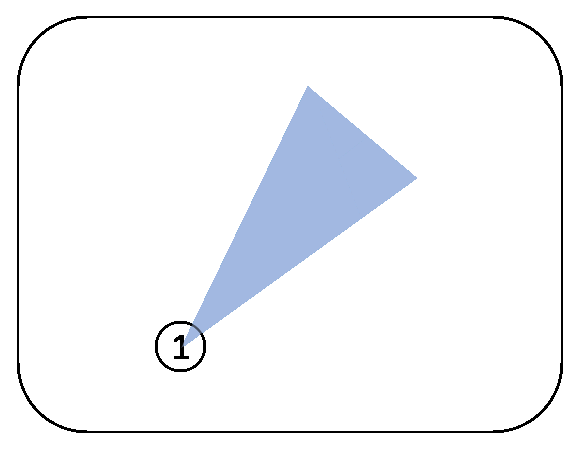
\includegraphics[width=1.0\linewidth]{sub6.eps}
  \caption{$F(S_A)$}
\end{subfigure}
\begin{subfigure}{.22\textwidth}
  \centering
  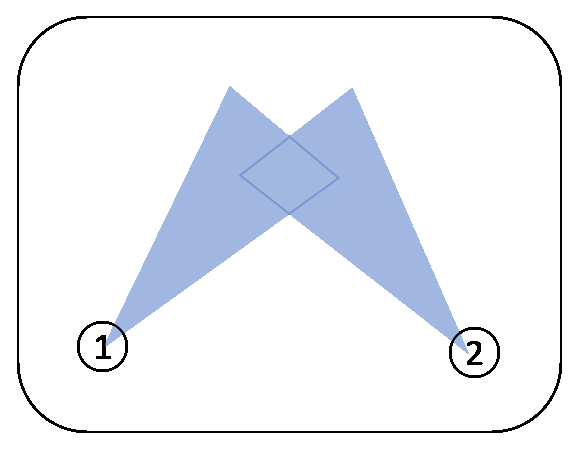
\includegraphics[width=1.0\linewidth]{sub7.eps}
  \caption{$F(S_B)$}
\end{subfigure}
\begin{subfigure}{.44\textwidth}
  \centering
  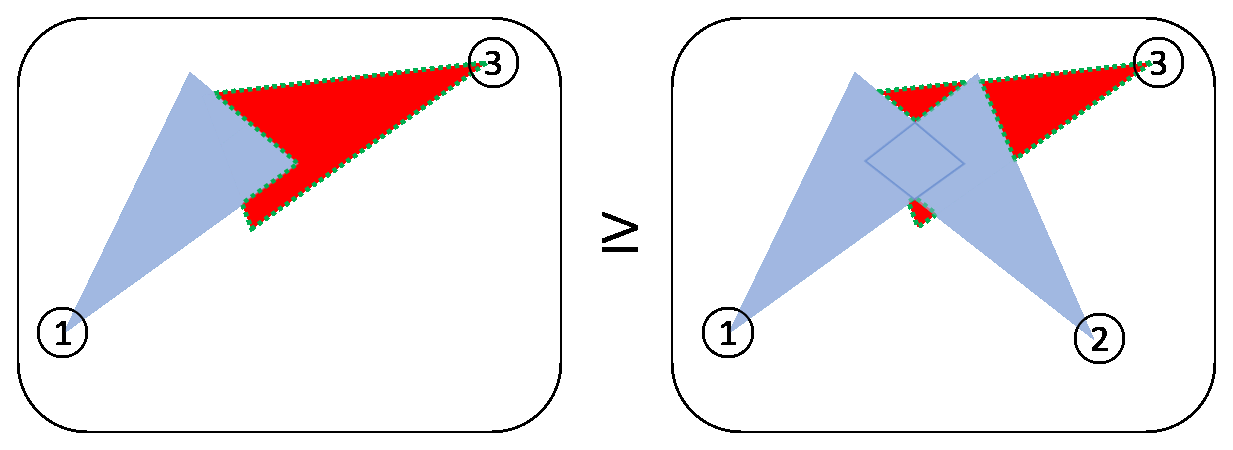
\includegraphics[width=1.0\linewidth]{sub5.eps}
  \caption{$F(S_A \cup s)-F(S_A)$ and $F(S_B \cup s)-F(S_B)$}
\end{subfigure}
\caption{Illustration of submodularity. The decimal number represents the selected sensor.
The colorful and white areas represent the covered and uncovered areas, respectively.
(a) $F(S_A)$ represents the covered area by $S_A,$ where $S_A = \{1\}.$ (b) $F(S_B)$ represents the covered area by $S_B,$ where $S_B = \{1, 2\}.$
(c) The green dash lines represent the submodular gain after adding $s,$ where $s = \{3\}.$ Left figure shows the $F(S_A\cup s) - F(S_A)$ and right figure shows that $F(S_B\cup s) - F(S_B).$}
\label{fig:submodularity}
 \end{center}
 \end{figure}

\section{Lower bound of GCB}
To further apply submodularity to routing constraints,
some definitions and the lower bound of GCB are introduced as follows:

\begin{definition}[Total curvature~\cite{conforti1984submodular}]
Given a finite set $S = \{1,2,...,N\},$
a monotone submodular function $f$, the total curvature of $f$ is defined as:

\begin{equation}
\kappa_f = 1 - \min_{s\in S:f(\{ s \}) > 0}\frac{f(S)-f(S \setminus\{ s \})}{f(\{ s \})}.
\label{eq:kappa}
\end{equation}

If the $\kappa_f = 0$, then $f$ is modular.
%Moreover, $\frac{1}{\alpha_f} \ge 1-\kappa_f \ge 0$ can be directly obtained from Def.~\ref{def:sub_ratio}~\cite{lin2023improvement}.
\label{def:kappa_f}
\end{definition}

\begin{definition}[The largest size of feasible solution $K_c$~\cite{zhang2016submodular}]
Given a ground set $S$ and cost function $c$, $K_c$ is defined as:

\begin{equation}
K_c = \max_{X\subseteq S}\{|X|\; | c(X) \le B\},
\end{equation}
where $B$ is budget.
\label{def:K_c}
\end{definition}

%\begin{theorem}[Lower bound of GCB~\cite{zhang2016submodular}]
%Given a submodular monotone set function $f$ and a monotone set function $c$,
%the GCB approach is to maximize f subject to the budget $B$.
%The GCB performance of a set X achieves
%\begin{equation}
%  f(X)\ge\frac{1}{2}(1-\frac{1}{e})f(\tilde{X}),
%\end{equation}
%where
%\begin{equation}
% \tilde{X} = arg\max _X\{
%f(X) | c(X)\le B\frac{ \alpha_{\hat{c}}(1 + \alpha_c^2 (K_c-1) (1-\kappa_c) )  }{ \psi(n) K_c }
%\}.
%\label{eq:noOPT}
%\end{equation}
%$c$ and $\hat{c}$ represent the cost function and the approximation cost function, respectively.
%The TSP solver is  $\psi(n)-$approximation (i.e. $c(X) \le \hat{c}(X) \le \psi(n)c(X),$ and $\psi(n) \ge 1$).
%
%\label{thm:GCB}
%\end{theorem}

\begin{theorem}[Lower bound of GCB under the tree-structured graph~\cite{lin2023improvement}]
Given a submodular monotone set function $f$ and a tree-structured graph cost function $c$,
the GCB approach is to maximize f subject to the budget $B$.
The performance of a set X achieves
\begin{equation}
  f(X)\ge\frac{1}{2}(1-\frac{1}{e})f(\overline{X}),
\end{equation}
where
\begin{equation}
 \overline{X} = \arg\max _X\{
f(X) | c(X)\le B(1-\kappa_c + \frac{\kappa_c}{K_c})
\}.
\label{eq:OPT_lin}
\end{equation}

\label{thm:GCB_lin}
\end{theorem}

\section{Prim and Dijkstra (PD) algorithm}

Minimum spanning tree is to minimize the total weight (TW) in a weighted undirected graph.
Prim's algorithm is a well-known greedy algorithm to find a minimum spanning tree for a weighted undirected graph~\cite{prim1957shortest}.
%The idea is to maintain two sets of vertices,
%the vertices in the MST and the vertices not in the MST.

Dijkstra algorithm is a well-known algorithm to find the shortest path between source node and terminal node in an undirected weighted graph.
Dijkstra algorithm is adopted for SPT to find the source point between the other nodes in graph.
To combine Prim and Dijkstra algorithms, the objective function is proposed as follows:

\begin{definition}[The objective function of Prim and Dijkstra algorithm~\cite{alpert1993direct}]
The $v_i$ and $v_j$ of Prim and Dijkstra algorithm are chosen to minimize
\begin{equation}
  \begin{aligned}
    (\alpha\cdot l_i)+d_{ij} \; s.t. \; v_j\in T, v_i \in V - T,
  \end{aligned}
  \label{eq:PD_obj}
\end{equation}
where $\alpha\in[0, 1]$ is a tuning parameter, $l_i$ is the length from source (start point) to node $v_i$, $d_{ij}$ is the distance between $v_i$ and $v_j$, $V$ is all vertices in graph and $T$ is current growing tree.
\end{definition}

Prim-Dijkstra (\emph{PD}) algorithm~\cite{alpert1993direct} can generate different types of spanning trees.
If $\alpha = 0$, PD algorithm is Prim algorithm; if $\alpha = 1$, PD algorithm is Dijkstra algorithm.
As Fig.~\ref{fig:PD_intro}(a) shows, there are six subgoals on this map.
As Fig.~\ref{fig:PD_intro}(b) shows, the Prim algorithm generates the minimum spanning tree (MST).
As Fig.~\ref{fig:PD_intro}(c) shows, the Dijkstra algorithm on this map generates the shortest path tree.
In the \emph{PD} algorithm, different parameters generate different spanning trees.
%For example,
%if $\alpha = 0$, PL = $13.969$ and TW = $5.393$ in Fig.~\ref{fig:PD_intro} (b).
%If $\alpha = 1$, PL = $7.658$ and TW = $7.658$ in Fig.~\ref{fig:PD_intro} (c).
%If $\alpha = 0.5$, PL = $8.119$ and TW = $6.726$ in Fig.~\ref{fig:PD_intro} (d).
%(c), these trees are edge cases generated by the \emph{PD} algorithm.
%{\color{olive}As Fig.~\ref{fig:PD_intro}(d) shows, the \emph{PD} algorithm in this map generates various spanning trees.
%This research analyzes the performances of different types of spanning trees.

%The inputs are an undirected graph ($G$), the source ($s$).
%The output is the spanning tree.
%Line $1$ is to build $Q$ (vertices in $G$).
%Line $2-3$ is initializing.
%Line $5$ is to find the distance connecting $v_q$ and $v_k$, where $v_q$ belongs to the current growing tree ($S$), and $v_k$ does not belong to the current growing tree {\color{olive}of the tree}.
%Line $6$ is to find the path length from {\color{olive}the} source vertex to $v_q$ along the current growing tree ($S$).
%Line $7$ is to trade off Prim algorithm and Dijkstra algorithm.
%{\color{olive}Line $8-9$ is to update current tree and spanning tree.}
%{\color{red} (How about plotting a figure to explain it. Here is background knowledge. )}


%The PD algorithm is to trade off between MST and SPT.
%The $\alpha$ is a weighting parameter that allows to span the entire tradeoff range.
%When $\alpha = 0$, the PD algorithm results in generating MST.
%When $\alpha = 1$, the PD algorithm results in generating SPT.



%\begin{algorithm}[ht]	
%	\KwIn{\\
%$G = (V, E, w)$: undirected graph \\
%$s$: the start point
%}
%\KwOut{$S$: spanning tree}
%\Parameter{$\alpha$ (between $0$ and $1$)}
%	\caption{Prim and Dijkstra algorithm}
%	\begin{algorithmic}[1]
%    \State {$Q = V$ \#all of vertices in $G$}
%    \State {$Q = Q \setminus \{s\}$}
%    \State {$S = \phi$}
%    \WHILE {$Q \neq \phi$}
%        \State {let $d_{qk}$ be the cost edge such that $q \in Q$ and $k \in V \setminus Q$}
%        \State {$pl_q$ is distance from source to $v_q$}
%        \State {minimize ($\alpha\times pl_i+d_{iu}$) where $i\in Q,$ $u\in V\setminus Q$}
%        \State {$Q = Q \setminus \{i\}$}
%        \State {$S = S \cup (u, i)$}
%    \ENDWHILE	
%    \end{algorithmic}	
%	\label{al:PD}
%\end{algorithm}

\begin{figure}[htbp]
 \begin{center}
\begin{subfigure}{.22\textwidth}
  \centering
  \includegraphics[width=1.0\linewidth]{pt.jpg}
  \caption{The complete graph}
\end{subfigure}
\begin{subfigure}{.22\textwidth}
  \centering
  \includegraphics[width=1.0\linewidth]{toy_alpha_00.jpg}
  \caption{MST ($\alpha=0$)}
\end{subfigure}
\begin{subfigure}{.22\textwidth}
  \centering
  \includegraphics[width=1.0\linewidth]{toy_alpha_10.jpg}
  \caption{SPT ($\alpha=1$)}
\end{subfigure}
\begin{subfigure}{.22\textwidth}
  \centering
  \includegraphics[width=1.0\linewidth]{toy_alpha_05.jpg}
  \caption{Tree $(\alpha=0.5)$}
\end{subfigure}
\caption{Illustration of the \emph{PD} algorithm. (a) The complete graph.
The blue points, blue edges and decimal numbers represent subgoals, paths and the index of subgoals, respectively.
(b) Minimum spanning tree (MST).
(c) Shortest path tree (SPT).
(d) The tree between MST and SPT. Tuning the $\alpha$ parameter generates different spanning trees.
}
\label{fig:PD_intro}
 \end{center}
 \end{figure}

\section{Extended probability of detection (EPD)}


IPP problems can be formulated as POMDP problems~\cite{kadane1977optimal}, which are NP-hard. Hence, probability of detection model is proposed.
However, the assumptions of probability of detection are not realistic, i.e., the agent only moves to neighbor cells, and the sensor has no overlapping covearge. The extended probability of detection (EPD) was proposed~\cite{tseng2016learning} to apply to real world.
The definition of EPD is as follows:

\begin{definition}[Extended probability of detection (EPD)~\cite{tseng2016learning}]
The agent gets the information $z$.
The assumptions of EPD are as follows:\\
(i) There is no target detection ($z = 1$) along the path.\\
(ii) The sensing overlapping is available.\\
(iii) The agent could move to any subgoals.\\
The equation of the cumulative EPD is defined as
\begin{equation}\label{eq:cepd}
  f_p(S_g) = \sum_{i=1}^{T}P(S_{g,i})\cdot g
\end{equation}
, where $f_p$ is the cumulative EPD along the path, $g$ is glimpse function and $P(S_{g,i})$ is the probability of covered cells at the i-th subgoal. The value of glimpse function can be calculated from the confusion table.

\end{definition}

As Fig.~\ref{fig:EPD_z} shows, the agent's sensing area is not fitting in its local cell.
Due to the availability of sensing overlap, the probability of sensing area is recomputed.
The assumption is that the agent moves along the path without any detections ($z=0$).
Finally, the agent can navigate to any subgoals instead of neighborhood areas.


%\begin{figure}[t!]
% \begin{center}
%  \centering
%  \includegraphics[width=0.5\linewidth]{EPD.jpg}
%\caption{Illustration of Extended probability of detection. The white and green areas represent low probability and high probability, respectively.  {\color{red} (you should plot the branches (z=1, z=0)?)}}
%\label{fig:EPD}
% \end{center}
% \end{figure}

\begin{figure}[htbp]
 \begin{center}
  \centering
  \includegraphics[width=0.5\linewidth]{EPD_z.jpg}
\caption{Illustration of no detection. In the PD assumption, the agent assumes there is no detection of a target along a path.}
\label{fig:EPD_z}
 \end{center}
 \end{figure}                % 第三章
\chapter{Problem Formulation}
Given a weighted graph $\mathcal{G}=(V, E, w)$ and an objective function $F:2^E \rightarrow \mathbb{R}^+$, where $V$ is a set of vertex, $E$ is a set of edges and $w:E \rightarrow \mathbb{R}^+$ is a distance function, the goal is to find a subset $S \subseteq E$ that maximizes environmental coverage and balances robot workloads subject to a constraint.
The objective function $F(S)=f(S)+\lambda \mathcal{B}(S)$ \cite{li2024mrsis} is defined as a linear combination of a coverage function $f$ and a balancing function $\mathcal{B}$, where $\lambda \in [0,1]$ is the weight of the balancing function\footnote{Both $f$ and $\mathcal{B}$ functions are normalized.}.
In 3D environments, the coverage function is defined by calculating the ratio of the number of covered voxels to the total number of environmental voxels.

Two variant formulations with known world maps are considered: Multi-robot search with independence system (MRSIS) \cite{li2024mrsis} and Multi-robot search with matroid (MRSM). \\

\section{Multi-robot search with independence system (MRSIS)}
\begin{problem} \label{prob:objective-IS}
    (MRSIS) \cite{li2024mrsis} Given an objective function $F$, a set of independence system $\mathit{\mathbb{I}} = \{I_G , I_C\}$, the number of robots $n \in \mathbb{N}^+$, and a set of routing constraints for each robot $l = \{l_i \in \mathbb{R}^+\}_{i=1}^n$, find a subset $S \subseteq E$ that maximizes $F$ under an intersection of independence systems
    \begin{equation} \label{eq:objective-IS}
        \begin{aligned}
            \max_{S} \quad & F(S) \\
            \textrm{s.t.} \quad & S \in \bigcap_{I \in \mathit{\mathbb{I}}} I,
        \end{aligned}
\end{equation}
\end{problem}

The intersection system $\bigcap_{I \in \mathit{\mathbb{I}}} I$ is defined as an intersection of all elements in the set of independence systems.
$\mathit{\mathbb{I}} = \{I_G , I_C\}$ is defined as a set of independence systems, where $I_G=(E, \mathcal{I}_G)$ models the robots' routing constraint and $I_C=(E, \mathcal{I}_C)$ models the cluster constraint.\\


The following theorems and corollaries prove that the routing and clustering constraints are $k$-independence systems.
Then, the theoretical performance guarantee of MRSIS \cite{li2024mrsis} is provided.


\begin{theorem} \label{thm:general-routing} (Routing constraint of a $k$-independence system)
The routing constraint for multiple robots $I_G=(E, \mathcal{I}_G)$ is a $k_G$-independence system, where $k_G > 1$. The independent set is defined as $\mathcal{I}_G=\{S \subseteq E : c(S \cap X_i) \leq l_i , \forall i\in \{1,...,n\}\}$, where $c:2^E \rightarrow \mathbb{R}^+$ is a routing cost function (e.g., TSP or MST solver), $X_i \subseteq S$ is the set of $i^{th}$ cluster and $l_i$ is a routing budget.
\end{theorem}
\begin{proof}
To prove that $I_G$ is an independence system, two properties described in Def. \ref{def:independence-system} must hold.

\textbf{(Non-emptiness property)} Consider a set $B_1=\emptyset$.
Let $A=\{1,...,n\}$ and $m_i=c(B_1 \cap X_i), \forall i\in A$ be the routing costs of the $i$-th cluster and $X_i$ be a set of cluster $i$. Since $B_1$ is an empty set, it implies that $m_i=0, \forall i\in A$. Thus, $B_1$ belongs to the independent set $\mathcal{I}_G$.

\textbf{(Downward closure property)} Consider a set $B_1\subseteq E$ and $B_1 \in \mathcal{I}_G$. Let $m_i=c(B_1 \cap X_i), \forall i\in A$ be the routing costs of the $i$-th cluster and $X_i$ be a set of cluster $i$.
Since $B_1 \in \mathcal{I}_G$, this implies that $c(B_1 \cap X_i) \leq l_i, \forall i\in A$. Therefore, $m_i \leq l_i, \forall i\in A$. Let $B_2 \subseteq B_1$ and $n_i=c(B_2 \cap X_i), \forall i\in A$. Since $B_2$ contains edges no more than $B_1$, the routing costs $n_i \leq m_i$. As a result, $n_i \leq m_i \leq l_i$. Therefore, $B_2$ belongs to the independent set $\mathcal{I}_G$.

Since the independent set $\mathcal{I}_G$ satisfies the non-emptiness and downward closure properties, $I_G=(E, \mathcal{I}_G)$ is a $k_G$-independence system. If $I_G$ does not satisfy the exchange property (Def. \ref{def-matroid}), $k_G$ will be greater than 1.

To prove that $k_G > 1$, consider two sets $B_1\in \mathcal{I}$ and $B_2 \in \mathcal{I}$, where $|B_1|>|B_2|$.
Let $s=B_1 \setminus B_2$, $m_i=c(B_1 \cap X_i)\leq l_i, \forall i\in A$ and $n_i=c(B_2 \cap X_i)=l_i, \forall i\in A$. If $X \notin \emptyset$, adding any element $x \in X$ to $B_2$ forms a new set $B_2'$. It is obvious that $B_2' \notin \mathcal{I}$ since $n_i=l_i \leq c(B_2' \cap X_i)$.
Therefore, $I_G$ does not satisfy the exchange property. $k_G$ is greater than 1.
\\
\end{proof}

\begin{corollary} \label{cor:clustering-indep-sys} (Clustering constraint as a $1$-independence system)
Let $E$ be an edge set and $S \subseteq E$ be a subset.
$I_C=(E, \mathcal{I}_C)$ is an $1$-independence system, where $\mathcal{I}_C=\{S \subseteq E : N \geq n \}$, $N$ is the number of clusters, and $n$ is the number of robots.
\end{corollary}
\begin{proof}
Since $I_C$ is a matroid (Thm. \ref{thm:clustering-matroid}) and matroid satisfies the properties of the independence system (Def. \ref{def:independence-system}),
the clustering constraint $I_C$ is an $1$-independence system.
\\
\end{proof}

\begin{theorem}  \label{def:independence-bound}
 (Lower bound of MRSIS\cite{li2024mrsis}) Let $F$ be the coverage and balancing function, $\mathit{\mathbb{I}}$ be a set of $k$-independence systems, $S$ be the solution of maximizing $F$ subject to the intersection of $\mathit{\mathbb{I}}$ via greedy algorithms. The performance of $S$ is
\begin{equation*}
      F(X) \geq \frac{1}{2+k_G} F(\overline{X^{opt}}),
\end{equation*}
where $k_G > 1$ and $\overline{X^{opt}}$ is an approximately optimal solution depending on the TSP or MST solver.
\end{theorem}
\begin{proof}
In Thm. \ref{thm:proposed-obj}, the coverage and balancing function $F$ satisfies the submodularity.
Let $\mathit{\mathbb{I}}=\{I_C, I_G\}$ be a set of $k$-independence systems. In Cor. \ref{cor:clustering-indep-sys}, the clustering constraint $I_C$ is a $1$-independence system. In Thm. \ref{thm:general-routing}, the general multi-robot routing constraint $I_G$ is a $k_G$-independence system.
By Thm. \ref{thm:intersection-k-systems}, the performance of MRSIS \cite{li2024mrsis} achieves $\frac{1}{2+k_G}\overline{OPT}$, where $\overline{OPT}$ is an approximately optimal solution that depends on the routing cost function.
\\
\end{proof}

To improve the performance of MRSIS \cite{li2024mrsis}, the set of independence systems is reformulated into the set of matroids.

\section{Multi-robot search with matroid (MRSM)}

\begin{problem} \label{prob:objective-Mat}
    (MRSM) Given an objective function $F$, a set of matroidal independence systems $\mathit{\mathbb{M}} = \{\mathcal{M}_R , \mathcal{M}_C\}$, the number of robots $n \in \mathbb{N}^+$, and a set of routing constraints for each robot $l = \{l_i \in \mathbb{R}^+\}_{i=1}^n$, find a set $S \subseteq E$ that maximizes $F$ under an intersection of matroidal independence systems
    \begin{equation} \label{eq:objective-Mat}
        \begin{aligned}
            \max_{S} \quad & F(S) \\
            \textrm{s.t.} \quad & S \in \bigcap_{\mathcal{M}\in \mathit{\mathbb{M}}} \mathcal{M},
        \end{aligned}
\end{equation}
\end{problem}

$\mathit{\mathbb{M}} = \{\mathcal{M}_R , \mathcal{M}_C\}$ is defined as a set of matroidal independence systems, where $\mathcal{M}_R=(E, \mathcal{I}_R)$ and $\mathcal{M}_C=(E, \mathcal{I}_C)$ are the robots routing constraint under tree structure and the clustering constraint, respectively.

The routing matroid $\mathcal{M}_R$ constrains the trajectory length of robots while constructing spanning trees.
The independent set $\mathcal{I}_R$ is a subset of $E$ which satisfies:
\begin{enumerate}
    \item $T \subset S$, where $T \subseteq E$ and $S \subseteq E$ are acyclic, and $|T| < |S|$,
    \item $c_{st}(S \cap X_i) \leq l_i , \forall i\in \{1,2,...,n\}$.
\end{enumerate}
where $X_i \subseteq S$ is the set of the $i^{th}$ cluster and $c_{st}:2^E \rightarrow \mathbb{R}^+$ is a routing cost function for a spanning tree.

The clustering matroid $\mathcal{M}_C$ is defined the same as in MRSIS \cite{li2024mrsis}.
The independent set $\mathcal{I}_C$ is defined as
\begin{align*}
    \mathcal{I}_C=\{S \subseteq E : N \geq n \},
\end{align*}
where $N$ is the number of clusters and $n$ is the number of robots. \\

The following Theorems introduce matroid constraints and the theoretical performance guarantee of MRSM.

\begin{theorem} \label{thm:routing-matroid} (Routing constraint under tree structure)
Let $E$ be an edge set and $T$ and $S$ be any subset of $E$. $\mathcal{I}_R$ is the set of subsets, $S\subseteq E$, which satisfies:
\begin{enumerate}
    \item $T \subset S$, where $T$ and $S$ are acyclic and $|T| < |S|$,
    \item $c_{st}(S \cap X_i) \leq l_i , \forall i\in \{1,...,n\}$, where $c_{st}:2^E \rightarrow \mathbb{R}^+$ is a routing cost function for a spanning tree, $X_i \subseteq S$ is the set of $i^{th}$ cluster and $l_i$ is a routing budget.
\end{enumerate}

The routing constraint $\mathcal{M}_R=(E, \mathcal{I}_R)$ is a matroid.
\end{theorem}
\begin{proof}
To prove that $\mathcal{M}_R$ is a matroid, two properties described in Def. \ref{def:matroid} must hold.

\textbf{(Downward closure property)} Consider a set $B_1\subseteq E$ and $B_1 \in \mathcal{I}_R$.
Let $A=\{1,...,n\}$ and $m_i=c_{st}(B_1 \cap X_i), \forall i\in A$ be the routing costs of the $i$-th cluster, and $X_i$ be the set of the $i$-th cluster.
Since $B_1 \in \mathcal{I}_R$, this implies that $B_1$ is a tree (acyclic graph) and $m_i \leq l_i, \forall i\in A$.
Let $B_2 \subseteq B_1$ and $n_i=c_{st}(B_2 \cap X_i), \forall i\in A$.
Since $B_2$ contains edges no more than $B_1$, the routing costs must be $n_i \leq m_i$.
In addition, removing any edge from $B_1$ forms $B_2$ which does not form a cycle.
As a result, $n_i \leq m_i \leq l_i$ and $B_2$ is acyclic.
Therefore, $\mathcal{I}_R$ satisfies the downward closure property.

\textbf{(Exchange property)} Consider two sets $B_1 \in \mathcal{I}_R$ and $B_2\in \mathcal{I}_R$, where $|B_1|>|B_2|$.
Since $B_1$ and $B_2$ satisfy the condition of the independent set and $|B_1|>|B_2|$, it implies that $B_2 \subset B_1$.
Let $m_i=c_{st}(B_1 \cap X_i)$ and $n_i=c_{st}(B_2 \cap X_i), \forall i\in A$.
If $B_2 \subset B_1$, it is clear that $n_i \leq m_i \leq l_i$.
Besides, removing any edge from $B_1$ forms $B_2$, which is acyclic.
Therefore, $\mathcal{I}_R$ satisfies the exchange property.

Since the independent set $\mathcal{I}_R$ satisfies the downward closure properties and the exchange property, $\mathcal{M}_R=(E, \mathcal{I}_R)$ is a matroid.\\
\end{proof}

\begin{definition}
    (Matroidal independence systems of routing and clustering constraints) Given a tree-structured routing constraint $\mathcal{M}_R$ with a set of routing budgets $\{l_i\}_{i=1}^n$ and a clustering constraint $\mathcal{M}_C$ with $n$ robots. A set of matroidal independence systems is defined as $\mathit{\mathbb{M}} = \{\mathcal{M}_R , \mathcal{M}_C\}$.\\
\end{definition}

The routing matroid $\mathcal{M}_R$ constrains the trajectory length of robots via constructing spanning trees while the clustering matroid $\mathcal{M}_C$ divides the ground set into groups for robots.

To illustrate the concept, two cases are illustrated as follows.
Fig. \ref{independent-set} illustrates the intersection system of $\mathcal{M}_R=(E, \mathcal{I}_R)$ and $\mathcal{M}_C=(E, \mathcal{I}_C)$.
Let $E$ be the set of edges between any vertex, $(a,b)\in E$ be an undirected edge, $\mathit{\mathbb{M}}=\{\mathcal{M}_R, \mathcal{M}_C\}$ be the set of matroidal independence systems, $l_i=10$ be the routing constraint and $n=3$ be the minimum number of clusters. In Fig. \ref{independent-set}(a), let $S_A=\{S_1,S_2,S_3\}$, where $S_1=\{(0,4)\},S_2=\{(3,5)\},$ and $S_3=\{(6,7),$$(7,8)\}$. $S_A$ satisfies the intersection system since $S_A$ is acyclic, $|S_A|\geq n$ and $c(S_A \cap S_i) \leq l_i$, where $i=\{1,2,3\}$.
In Fig. \ref{independent-set}(b), let $S_B=\{S_1,S_2\}$, where $S_1=\{(0,4),(4,2),(2,5),(3,5)\}$ and $S_2=\{(6,7),$$(7,8)\}$. $S_B$ does not satisfy the intersection system since $|S_B| < n$ and $c(S_B \cap S_1) > l_i$. \\

\begin{figure}
    \centering
    \begin{subfigure}[b]{0.4\textwidth}
        \includegraphics[width=1\textwidth]{mat-1.png}
        \caption{$S_A \in \bigcap_{\mathcal{M}\in \mathit{\mathbb{M}}} \mathcal{M}$}
    \end{subfigure}
    \hfill
    \quad
    \begin{subfigure}[b]{0.4\textwidth}
    \centering
        \includegraphics[width=1\textwidth]{mat-2.png}
        \caption{$S_B \not \in \bigcap_{\mathcal{M}\in \mathit{\mathbb{M}}} \mathcal{M}$}
    \end{subfigure}

    \caption{Illustration of the intersection system.
    The vertices and lines represent the subgoals and the distances between two vertices, respectively.
    Each color line denotes a cluster. (a) $S_A$ contains three clusters that satisfy the condition of the intersection system. (b) $S_B$ contains two clusters that violate the condition of the intersection system due to the under-budget of the clustering and the over-budget of routing constraints.
    }
    \label{independent-set}
\end{figure}

\begin{theorem}  \label{def:proposed-bound}
 (Lower bound of the proposed algorithm for MRSM) Let $F$ be the coverage and balancing function, $\mathit{\mathbb{M}}$ be a set of matroidal independence systems, $S$ be the solution of maximizing $F$ subject to the intersection of $\mathit{\mathbb{M}}$ via greedy algorithms. The performance of $S$ is
\begin{equation*}
      F(X) \geq \frac{1}{3} F(\widetilde{X^{opt}}),
\end{equation*}
where $\widetilde{X^{opt}}$ is the optimal solution under tree structure.
\end{theorem}
\begin{proof}
The coverage and balancing function $F$ is submodular (Thm. \ref{thm:proposed-obj}) and each element in $\mathit{\mathbb{M}}$ is a matroid (Thm. \ref{thm:clustering-matroid} and Thm. \ref{thm:routing-matroid}).
By Thm. \ref{thm:intersection-matroid-bound}, the performance of the proposed method is guaranteed to find a solution that achieves $\frac{1}{3}\widetilde{OPT}$, where $\widetilde{OPT}$ is the optimal performance under tree structure.
\end{proof}

               % 第四章
\chapter{Proposed algorithms}
There are two algorithms: CBST algorithm and terrain monitoring algorithm.
The Alg.~\ref{al:CBST} is to generate the CBST (e.g., from Fig.~\ref{fig:method_intro} (a) to Fig.~\ref{fig:method_intro} (b)).
The Alg.~\ref{al:TM_CBST} is to generate the path using GCB algorithm (e.g.,  from Fig.~\ref{fig:method_intro} (b) to Fig.~\ref{fig:method_intro} (c)).


In Alg.~\ref{al:CBST}, the inputs are an undirected graph ($G$), the source ($s$).
The output is the spanning tree.
Line $1$ is to build $Q$ (vertices in $G$).
Lines $2-3$ are initialization{\color{olive}s}.
Line $5$ is to find the distance connecting $v_q$ and $v_k$, where $v_q$ belongs to the current growing tree ($S$), and $v_k$ does not belong to the tree current growing tree.
Line $6$ is to find the path length from the source vertex to $v_q$ along the current growing tree ($S$).
Line $7$ is to maximize $f/c$, where $c$ is the cost function about Prim's algorithm and Dijkstra algorithm.
Lines $8-9$ are to update current tree and spanning tree.


\begin{algorithm}[htbp]	
	\KwIn{\\
$G = (V, E, w)$: undirected graph \\
$s$: the start point \\
$f$: objective function
}
\KwOut{$S$: spanning tree}
\Parameter{$\alpha$ (between $0$ and $1$)}
	\caption{Cost-benefit spanning tree}
	\begin{algorithmic}[1]
    \State {$Q = V$ \#all of vertices in $G$}
    \State {$Q = Q \setminus \{s\}$}
    \State {$S = \phi$}
    \WHILE {$Q \neq \phi$}
        \State {let $d_{qk}$ be the cost edge \; such that $q \in Q$ and $k \in V \setminus Q$}
        \State {$pl_q$ is distance from source to $v_q$}
        \State {maximize ($\frac{f}{\alpha\times pl_i+d_{iu}}$) where $i\in Q,$ $u\in V\setminus Q$}
        \State {$Q = Q \setminus \{i\}$}
%        \FOR {$u$ which are neighbors of $i$ still in $Q$}
%            \State {$RELAX(u, i, w)$}
            \State {$S = S \cup (u, i)$}
%        \ENDFOR
    \ENDWHILE	
    \end{algorithmic}	
	\label{al:CBST}
\end{algorithm}

\begin{algorithm}[thbp]
\KwIn{\\
$S=(V, E, w)$: spanning tree \\
$s$: the start point \\
$f$: objective function \\
$c$: cost function from spanning tree $S$ \\
$B$: budget
}
\KwOut{$\pi$: subgoal set}
    \caption{Terrain monitoring using CBST}
    \begin{algorithmic}[1]
    \State {$G:=\phi$}
    \State {$\pi:=\phi$}
    \State {$V^{'} = V$}
    \WHILE {$V^{'}\neq \phi$}
        \FOR {$X \in V$}
            \State {$\Delta_f^X:=f(G\cup X)-f(G)$}
            \State {$\Delta_c^X:=c(G\cup X)-c(G)$}
        \ENDFOR
        \State {$X^* = argmax\{\frac{\Delta_f^X}{\Delta_c^X}\}$}
        \IF {$c(G\cup X^*)\le B$}
            \State {$\pi = \pi\cup X^*$}
        \ENDIF
        \State {$V^{'}=V^{'}\setminus X^*$}
    \ENDWHILE
    \end{algorithmic}
    \label{al:TM_CBST}
\end{algorithm}

In Alg.~\ref{al:TM_CBST}, the inputs, $S$, $s$, $f$, $c$, and $B,$ represent spanning tree built from Alg.~\ref{al:CBST}, the start point, objective function, cost function from spanning tree $S$ using shortest path tree, and a cost budget, respectively.
The output is $\pi$ which is the subgoal set with budget constraint.
Lines $1-3$ are initializations.
Lines $4-9$ are to find maximum cost-benefit point in the spanning tree.
Lines $10-12$ are to pick the point subject to budget constraint.
Line $13$ is to avoid that the agent pick{\color{olive}s} the point repeatedly.               % 第五章
\chapter{Experiments}
To evaluate the performance of different approaches, there are three experiments:
the maximization extended probability of detection problem, the search problem, and Tuning $\alpha$ parameters.
The EX$1$ is to evaluate the extended probability of target detection (EPD) of different offline approaches with routing constraints in simulations.
The EX$2$ is to evaluate the search time of different approaches with routing constraints in simulations and real world.
%The EX$3$ is to evaluate the search time of changing the parameter $\alpha$ in CBST {\color{olive}to verify wether the $\alpha$ changing will influence results}.
The purpose of EX3 is to evaluate the influence of changing $\alpha$ for search results.

\section{Experiment setup}
In the EX$1$ and EX$2$, there are two different size maps.
The size of  map 1 and map 2 are  $4 \times 4 \times 3$ $(m^3)$ and $8 \times 8 \times 3$ $(m^3)$, respectively.
As shown in Fig.~\ref{fig:Ground_set}, the ground set $S$ is generated with $||S|| = 58.$
The numbers of subgoals in low altitude is more than that in high altitude, due to the camera field of view (FOV).
The index $1$ is start point.
The experimental setup (e.g., camera and drone parameters) is as shown in Table~\ref{tab:drone_info}.
%The minimum altitude, the maximum altitude and the distance between altitude levels are $0.5,$ $3.0$ and $0.3$, respectively.

%The index $1$ in Fig.~\ref{fig:Ground_set} is the start point.
%The minimum altitude in Fig.~\ref{fig:Ground_set} is $0.5;$ the maximum altitude in Fig.~\ref{fig:Ground_set} is $3.0.$
%The distance between altitude levels on the subgoals is $0.3.$
The cost constraints are $10$ and $40,$ respectively.
The cost function $c$ is measured by Euclidean distance.
Note that, since computing routing cost is NP-hard problem, $c$ is approximated by $\hat{c}$ via Nearest Neighbor (NN) algorithm~\cite{rosenkrantz1977analysis} which provides a $\frac{3}{2}-$approximation factor.
%The experimental parameters are at Table.~\ref{tab:cam_info}.
%The range of downward camera is $3.0 (m).$ {\color{olive}Its} horizontal FOV is $60^{\circ}$;
%{\color{olive}its} vertical FOV is $45^{\circ}.$
%{\color{olive}Its} frame rate per second is $10.$
%It represents the camera takes $10$ frames per second.



\begin{table}[htbp]
   \caption{Drone hardware setup in simulation.}
   \begin{center}
     \begin{tabular}{|| c | l | l ||}
     \hline
     Parameter & description & value\\ [0.5ex]
     \hline\hline
     $c_r$ & range & $3.0$ (m) \\
     \hline
     $FOV_h$ & horizontal FOV & $60^{\circ}$ \\
     \hline
     $FOV_v$ & vertical FOV & $45^{\circ}$ \\
     \hline
     $c_{fr}$ & frame rate & $10$ (FPS) \\
     \hline\hline
     $h_{max}$ & flight minimum altitude & $0.5$ (m) \\
     \hline
     $h_{min}$ & flight maximum altitude & $3.0$ (m) \\
     \hline
     $h_{level}$ & flight altitude levels & $0.3$ (m) \\
     \hline
     $\omega_{max}$ & limitation of angular velocity & $42$ (deg/s) \\
     \hline
     $v_{max}$ & limitation of linear velocity & $1$ (m/s) \\
     \hline
    \end{tabular}
   \end{center}
   \label{tab:drone_info}
\end{table}

The target locates in $121$ places uniformly. The drone searches $5$ times in each place.
Hence, there are $605$ times.
The search processing is as follows: The agent takes off and moves to the next subgoal.
If the drone cannot find the target ($P(Z=1) \le 95 \%$), the agent will go through the next path (point) until finding the target ($P(Z=1)\ge 95 \%$) or utilizing all budgets.

There are two setups in the search experiments.
One is offline, the other one is online.
The online approach for the drone is to computes the information to decide the next subgoal(s);
the offline approach for the drone is to compute all subgoals before taking off.
There are two steps in the offline setup.
First, the path is generated by algorithm subject to budget constraints offline.
Second, the agent flies through the path.
There are three steps in the online setup.
First, the path (or the point) is generated by algorithm online.
Second, the agent flies through the path.
Third, the agent repeats first step via new measurements by second step until the terminal condition.

Along with path, the agent updates the probability of target detection ($Z$) in grid map via Bayesian filter.
There are $20 \times 20$ and $40 \times 40$ grids in map 1 and 2, respectively.
When the probability of the cell in grid map is greater than $95\%$ ($P(Z = 1)\ge 95 \%$), the agent finds the target.
Once the agent finds the target, it will land, and the search time is from taking off to landing.
$E[TTD^+]$ denotes the expected time till positive decisions~\cite{chung2011analysis}.

%{\color{olive}There are two terminal conditions.
%One is the agent finds the target ($P(Z = 1)\ge 95 \%$) subject to the budget constraint, the other one is the agent does not find the target {\color{olive}($P(Z = 1)\le 95 \%$)} until utilizing all budget.
%}

\begin{figure}[htbp]
  \centering
  \includegraphics[width=1.0\linewidth]{Ground_set.jpg}
  \caption{Ground set in simulation.}
  \label{fig:Ground_set}
\end{figure}

The map in the real world is a $4\times 4 \times 2 (m^3)$ lobby at the Mathematics department of National Central University (see Fig.~\ref{fig:lobby} (a)).
The target locates in 5 places randomly.
The drone searches 5 times in each place.
Hence, there are 125 times.
The budget $B=10 (m)$ is adopted in this map.
Fig.~\ref{fig:lobby} (a) shows the ground set $|S| = 31$ and the fixed start point is the subgoal $1$.
The target locates in three positions (blue stars) at each search.
%{\color{red} (add 3F experiments!)}
%The drone searches for the target 1 times at each location. %({\color{red}To do (5 times at each location)}).

As shown in Fig.~\ref{fig:nx}, the TD450 is developed by Taiwan Drone 100.
The D435i RGBD camera is to explore the environment while T265 camera is to localize itself.
The YOLOv5~\cite{glenn_jocher_2022_7347926} is adopted to detect objects running on NVIDA Jetson Xavier NX (see Fig.~\ref{fig:lobby} (b)).
The drone's operating system is Ubuntu 18.04 and runs the Robot Operating System (ROS).
The parameters of TD450 hardware setup are shown in Table~\ref{tab:drone_info_nx}.

\begin{table}[htbp]
   \caption{Drone hardware setup in real world.}
   \begin{center}
     \begin{tabular}{|| c | l | l ||}
     \hline
     Parameter & description & value\\ [0.5ex]
     \hline\hline
     $c_r$ & range & $3.0$ (m) \\
     \hline
     $FOV_h$ & horizontal FOV & $69^{\circ}$ \\
     \hline
     $FOV_v$ & vertical FOV & $42^{\circ}$ \\
     \hline
     $c_{fr}$ & frame rate & $30$ (FPS) \\
     \hline\hline
     $h_{max}$ & flight minimum altitude & $1.1$ (m) \\
     \hline
     $h_{min}$ & flight maximum altitude & $2.0$ (m) \\
     \hline
     $h_{level}$ & flight altitude levels & $0.3$ (m) \\
     \hline
     $\omega_{max}$ & limitation of angular velocity & $120$ (deg/s) \\
     \hline
     $v_{max}$ & limitation of linear velocity & $0.2$ (m/s) \\
     \hline
    \end{tabular}
   \end{center}
   \label{tab:drone_info_nx}
\end{table}


\begin{figure}[htbp]
  \centering
  \begin{subfigure}{.4\textwidth}
  \centering
  \includegraphics[width=1.0\linewidth]{lobby_and_subgoals.jpg}
  \caption{The lobby environment.}
\end{subfigure}
%\begin{subfigure}{.4\textwidth}
%  \centering
%  \includegraphics[width=1.0\linewidth]{lobby_sub.jpg}
%  \caption{{\color{olive}Ground set and target locations in real world.}}
%\end{subfigure}
\begin{subfigure}{.4\textwidth}
  \centering
  \includegraphics[width=1.0\linewidth]{det.jpg}
  \caption{The detection outcome of YOLOv5.}
\end{subfigure}
  \caption{(a)
  The black points, black decimal numbers,the index 1 in black represent the subgoals, the subgoal indexes and the source node, respectively.
  The blue stars and decimal numbers represent the target locations and the subgoal indexes, respectively.
  (b) The d435i provides the RGB images. The YOLOv5 detects the target in the image. The blue box represents the target location in the image with the detection probability.
  }
  \label{fig:lobby}
\end{figure}

\begin{figure}[htbp]
  \centering
  \includegraphics[width=1.0\linewidth]{nx.jpg}
  \caption{The TD450, sensors and development board.}
  \label{fig:nx}
\end{figure}

\section{EX$1$: EPD maximization}


In the experiment, the GCB-CBST is compared with four methods: A-optimality with CMA-ES~\cite{popovic2020informative}, GCB~\cite{zhang2016submodular}, GCB-MST~\cite{lin2023improvement}, and GCB-SPT. CMA-ES is online method, the others are offline methods.


The experiment results in the Gazebo simulation are summarized in Table~\ref{tab:EPD_map}.
Since CMA-ES is online algorithm, the accumulated EPD is not available.
GCB-CBST outperforms other approaches in the accumulated EPD in map 1 and 2.
The tree structures of MST, SPT, and CBST in map 1 and 2 are shown in Fig.~\ref{fig:TSG_map1} and~\ref{fig:TSG_map2}, respectively.
As shown in Fig.~\ref{fig:TSG_map1} (b) and~\ref{fig:TSG_map2} (b),
the tree structure of SPT are inefficient seeing due to the repeated paths.
Since the path in GCB-SPT have high cost-benefit, the accumulated EPD of GCB-SPT is higher than GCB-MST.
%The performance in GCB-CBST is better than that in GCB-MST because the agent will go through the repeated path.
These experiments show that GCB-CBST outperforms the other three methods in the maximal EPD problem.

%The GCB-TSG (MST) is worst case because the agent cannot go through the key point ($v_{58}$ in Fig.~\ref{fig:Ground_set}) that represents the agent will get lots of EPD in this map in Fig.~\ref{fig:TSG_map1}(a),~\ref{fig:TSG_map2}(a).
%As shown in~\ref{fig:TSG_map1}(b),~\ref{fig:TSG_map2}(b), the height of the GCB-TSG (SPT) is $1,$ so the agent will go through the next subgoal and go back to start point recursively. The agent in GCB-TSG (SPT) can go through the key point but wasting resources. The performance in GCB-TSG (SPT) is in median.
%{\color{red} (Read some papers. Check out how to describe the proposed approach is better than others.)}


%\begin{table}[t!]
%   \caption{EPD maximization experiment results in $4\times 4\times 3 (m)$ environment.}
%   \begin{center}
%     \begin{tabular}{| l | l | l | l | l | l |  l | l |} \hline
%     Method & accumulated EPD\\ \hline
%     A-opt with CMA-ES  & NA \\ \hline
%     GCB & $\textbf{0.993}$ \\ \hline
%     GCB-TSG(CBST) & $\textbf{0.958}$ \\ \hline
%     GCB-TSG(MST) & 0.489 \\ \hline
%     GCB-TSG(SPT) & 0.843 \\ \hline
%    \end{tabular}
%   \end{center}
%   \label{tab:EPD_map1}
%\end{table}

\begin{table}[htbp]
   \caption{
   EPD maximization experiment results.
   The accumulated EPD (AEPD) as follows.
   % in $8\times 8\times 3 (m)$ environment.
   }
   \begin{center}
     \begin{tabular}{| c | l | l | l | l | l |  l | l |} \hline
     Method & AEPD (map1) & AEPD (map2)\\ \hline
     A-opt with CMA-ES  & NA & NA \\ \hline
     GCB           & 0.90 & 0.80\\ \hline
     GCB-CBST & $\textbf{0.99}$ & $\textbf{0.84}$ \\ \hline
     GCB-MST  & 0.489 & 0.47 \\ \hline
     GCB-SPT  & 0.843 & 0.52 \\ \hline
%     2 & A-opt with CMA-ES  & NA \\ \hline
%     2 & GCB            & 0.80 \\ \hline
%     2 & GCB-CBST & $\textbf{0.84}$ \\ \hline
%     2 & GCB-MST  & 0.47 \\ \hline
%     2 & GCB-SPT  & 0.52 \\ \hline
    \end{tabular}
   \end{center}
   \label{tab:EPD_map}
\end{table}

\begin{figure}[htbp]
 \begin{center}
\begin{subfigure}{.45\textwidth}
  \centering
  \includegraphics[width=1.0\linewidth]{mst_map1.jpg}
  \caption{The tree structure of MST}
\end{subfigure}
\begin{subfigure}{.45\textwidth}
  \centering
  \includegraphics[width=1.0\linewidth]{spt_map1.jpg}
  \caption{The tree structure of SPT}
\end{subfigure}
\begin{subfigure}{.45\textwidth}
  \centering
  \includegraphics[width=1.0\linewidth]{f_c_map1.jpg}
  \caption{The tree structure of CBST}
\end{subfigure}
\caption{The blue circles represent the ground set, the green circle represent the picked subgoals, and the red lines represent the path, respectively. There are three tree structures in map1.}
\label{fig:TSG_map1}
 \end{center}
 \end{figure}

\begin{figure}[htbp]
 \begin{center}
\begin{subfigure}{.45\textwidth}
  \centering
  \includegraphics[width=1.0\linewidth]{mst_map2.jpg}
  \caption{The tree structure of MST}
\end{subfigure}
\begin{subfigure}{.45\textwidth}
  \centering
  \includegraphics[width=1.0\linewidth]{spt_map2.jpg}
  \caption{The tree structure of SPT}
\end{subfigure}
\begin{subfigure}{.45\textwidth}
  \centering
  \includegraphics[width=1.0\linewidth]{f_c_map2.jpg}
  \caption{The tree structure of CBST}
\end{subfigure}
\caption{The blue circles represent the ground set, the green circle represent the picked subgoals, and the red lines represent the path, respectively. There are three tree structures in map2.}
\label{fig:TSG_map2}
 \end{center}
 \end{figure}


\section{EX$2$: Search experiment}

The goal of the drone is to find the target as soon as possible subject to budget constraint, so the metrics in this experiment are expected time till positive decisions ($\mathbb{E}$[TTD$^+$]) and success rate.

The parameters are same as EX$1$.

\subsection{Simulation}
To evaluate the search performance, the expected time till positive decision ($\mathbb{E}$[TTD$^+$]) is compared (see Fig.~\ref{fig:ETTD_map1} and~\ref{fig:ETTD_map2}).
GCB-CBST outperforms other four methods in $\mathbb{E}$[TTD$^+$].
GCB-CBST and GCB-SPT are competitive in map 1 since the drone moves to high cost-benefit subgoals.
However, the success rate in GCB-SPT is less than that in GCB-CBST since the path in GCB-SPT is inefficient.
% $\cong$ GCB-TSG (SPT) $\le$ GCB $\cong$ A-opt with CMA-ES $\le$ GCB-TSG (SPT);
%accuracy: GCB $\ge$ GCB-TSG (CBST) $\ge$ GCB-TSG (SPT) $\ge$ A-opt with CMA-ES $\ge$ GCB-TSG (MST).
%
%{\color{blue}The E[TTD$^+$] of GCB-CBST and SPT are better than that of GCB.
%The drone moves to the important subgoal at the first step along the paths obtained by the GCB-CBST and the GCB-SPT.
%Hence, the drone finds the target quickly.
%}


The success rates of the GCB and GCB-CBST are competitive in map 2 (see Table~\ref{tab:ETTD_map}).
The success rate of the GCB is higher than that of the GCB-CBST in map 1 (see Table~\ref{tab:ETTD_map}).
In the GCB-CBST path, the drone moves to the repeated subgoals. Hence, it has fewer false detections than GCB does.
GCB-CBST attains the a little less success rate than GCB in map1 because the drone moves to the repeated subgoals in GCB-CBST.

%The GCB-TSG (MST) is the worst case in E[TTD$^+$] and accuracy.
%The GCB-TSG (CBST) and GCB-TSG (SPT) outperform other three method in E[TTD$^+$].
%However, the path in GCB-TSG (SPT) is short, the accuracy in GCB-TSG (SPT) is worse than GCB-TSG (CBST) and GCB. The GCB is better than GCB-TSG (CBST) in accuracy.
In summary, GCB-CBST is the best method for search tasks, since it can move through the high cost-benefit subgoals immediately and repeatedly.


%{\color{olive}As shown in Table~\ref{tab:ETTD_map2}, the results are similar to Table.~\ref{tab:ETTD_map1}. The difference lies in the fact that previously important points have become relatively less important, resulting in poorer performance of GCB-TSG (SPT).
%On the other hand, GCB-TSG (CBST) still outperforms GCB in terms of E[TTD$^+$].
%}

\begin{table}[htbp]
   \caption{Search experiment results reveal indicators success rate and $\mathbb{E}$[TTD$^+$] in map1 and map2. }
   \begin{center}
     \begin{tabular}{| c | l | l | l | l | l |  l | l |} \hline
      \multirow{2}{*}{Method} & \multicolumn{2}{c|}{Map1} & \multicolumn{2}{c|}{Map2}\\ \cline{2-5}
        & $\mathbb{E}$[TTD$^+$] & success rate & $\mathbb{E}$[TTD$^+$] & success rate\\ \hline\hline
       CMA-ES  & 12.6  & 0.77& 85.7  & 0.28\\ \hline
      GCB & 12.6  & $\textbf{0.96}$ & 30.4  & $\textbf{0.73}$ \\ \hline
      GCB-CBST & $\textbf{5.9}$  & 0.8& $\textbf{26.9}$  & 0.705\\ \hline
      GCB-MST & 18.4 & 0.44  & 48.3 & 0.30 \\ \hline
      GCB-SPT & 6.0 & 0.75 & 30.5 & 0.43\\ \hline
%     2 & A-opt with CMA-ES  & 85.7  & 0.28\\ \hline
%     2 & GCB & 30.4  & $\textbf{0.73}$ \\ \hline
%     2 & GCB-CBST & $\textbf{26.9}$  & 0.70\\ \hline
%     2 & GCB-MST & 48.3 & 0.30 \\ \hline
%     2 & GCB-SPT & 30.5 & 0.43 \\ \hline
    \end{tabular}
   \end{center}
   \label{tab:ETTD_map}
\end{table}

\begin{figure}[htbp]
 \begin{center}
\begin{subfigure}{.30\textwidth}
  \centering
  \includegraphics[width=1.0\linewidth]{GCB_CBST_ETTD_map1.jpg}
  \caption{$\mathbb{E}[TTD]$ of GCB-CBST}
\end{subfigure}
\begin{subfigure}{.30\textwidth}
  \centering
  \includegraphics[width=1.0\linewidth]{GCB_SPT_ETTD_map1.jpg}
  \caption{$\mathbb{E}[TTD]$ of GCB-SPT}
\end{subfigure}
\begin{subfigure}{.30\textwidth}
  \centering
  \includegraphics[width=1.0\linewidth]{GCB_MST_ETTD_map1.jpg}
  \caption{$\mathbb{E}[TTD]$ of GCB-MST}
\end{subfigure}
\begin{subfigure}{.30\textwidth}
  \centering
  \includegraphics[width=1.0\linewidth]{GCB_ETTD_map1.jpg}
  \caption{$\mathbb{E}[TTD]$ of GCB}
\end{subfigure}
\begin{subfigure}{.30\textwidth}
  \centering
  \includegraphics[width=1.0\linewidth]{A_ETTD_map1.jpg}
  \caption{$\mathbb{E}[TTD]$ of CMA-ES}
\end{subfigure}
\caption{$\mathbb{E}[TTD]$ of different tree-structured cost in map1. The x-axis and y-axis represent time (s) and probability, respectively.}
\label{fig:ETTD_map1}
 \end{center}
 \end{figure}

\begin{figure}[htbp]
 \begin{center}
\begin{subfigure}{.30\textwidth}
  \centering
  \includegraphics[width=1.0\linewidth]{GCB_CBST_ETTD_map2.jpg}
  \caption{$\mathbb{E}[TTD]$ of GCB-CBST}
\end{subfigure}
\begin{subfigure}{.30\textwidth}
  \centering
  \includegraphics[width=1.0\linewidth]{GCB_SPT_ETTD_map2.jpg}
  \caption{$\mathbb{E}[TTD]$ of GCB-SPT}
\end{subfigure}
\begin{subfigure}{.30\textwidth}
  \centering
  \includegraphics[width=1.0\linewidth]{GCB_MST_ETTD_map2.jpg}
  \caption{$\mathbb{E}[TTD]$ of GCB-MST}
\end{subfigure}
\begin{subfigure}{.30\textwidth}
  \centering
  \includegraphics[width=1.0\linewidth]{GCB_ETTD_map2.jpg}
  \caption{$\mathbb{E}[TTD]$ of GCB}
\end{subfigure}
\begin{subfigure}{.30\textwidth}
  \centering
  \includegraphics[width=1.0\linewidth]{A_ETTD_map2.jpg}
  \caption{$\mathbb{E}[TTD]$ of CMA-ES}
\end{subfigure}
\caption{$\mathbb{E}[TTD]$ of different tree-structured cost in map2. The x-axis and y-axis represent time (s) and probability, respectively.}
\label{fig:ETTD_map2}
 \end{center}
 \end{figure}
\clearpage
\subsection{Real world}
The tree structures of GCB-CBST, GCB-MST, and GCB-SPT are shown in Fig.~\ref{fig:TSG_lobby}.
GCB-CBST outperforms the other four methods in $\mathbb{E}$[TTD$^+$] (see Table~\ref{tab:ETTD_lobby}).
The height in real world is lower than that in the simulation,
so the path in GCB-SPT does not have high coverage.
The $\mathbb{E}$[TTD$^+$] in GCB-SPT is the worst.

The GCB-CBST outperforms the other four methods in success rate (see Table~\ref{tab:ETTD_lobby}),
since the GCB-CBST must go to subgoals via tree structure, and the drone moves to the repeated subgoals which have high cost-benefit values.
The GCB-MST and GCB-SPT are the worst in success rate.

These experiments show that GCB-CBST outperforms the other four benchmarks in search problems.

\begin{table}[htbp]
   \caption{Search experiment results reveal indicators success rate and $\mathbb{E}$[TTD$^+$] in real world. }
   \begin{center}
     \begin{tabular}{| c | l | l | l | l | l |  l | l |} \hline
      %\multirow{2}{*}{Method} & \multicolumn{2}{c|}{Map1} & \multicolumn{2}{c|}{Map2}\\ \cline{2-5}
        & $\mathbb{E}$[TTD$^+$] & success rate\\ \hline\hline
      CMA-ES  & 86.91 & 0.88\\ \hline
      GCB     & 69.23  & 0.88\\ \hline
      GCB-CBST& $\textbf{51.92}$ & $\textbf{1.00}$\\ \hline
      GCB-MST & 68.77  & 0.52\\ \hline
      GCB-SPT & 79.59  & 0.68\\ \hline
%     2 & A-opt with CMA-ES  & 85.7  & 0.28\\ \hline
%     2 & GCB & 30.4  & $\textbf{0.73}$ \\ \hline
%     2 & GCB-CBST & $\textbf{26.9}$  & 0.70\\ \hline
%     2 & GCB-MST & 48.3 & 0.30 \\ \hline
%     2 & GCB-SPT & 30.5 & 0.43 \\ \hline
    \end{tabular}
   \end{center}
   \label{tab:ETTD_lobby}
\end{table}

\begin{figure}[htbp]
 \begin{center}
\begin{subfigure}{.45\textwidth}
  \centering
  \includegraphics[width=1.0\linewidth]{lobby_mst_10.jpg}
  \caption{The tree structure of MST}
\end{subfigure}
\begin{subfigure}{.45\textwidth}
  \centering
  \includegraphics[width=1.0\linewidth]{lobby_spt_10.jpg}
  \caption{The tree structure of SPT}
\end{subfigure}
\begin{subfigure}{.45\textwidth}
  \centering
  \includegraphics[width=1.0\linewidth]{lobby_cbst_10.jpg}
  \caption{The tree structure of CBST}
\end{subfigure}
\caption{Three tree structures in the lobby environment.
The blue circles and green circles represent the ground set and the picked subgoals, respectively.
The red lines represent the paths. }
\label{fig:TSG_lobby}
 \end{center}
 \end{figure}







%\begin{table}[t!]
%   \caption{Search experiment results in $8\times 8\times 3 (m)$ environment.
%   {\color{red} (merge these two table using map 1 and map 2.)}
%   }
%   \begin{center}
%     \begin{tabular}{| l | l | l | l | l | l |  l | l |} \hline
%     Method & E[TTD$^+$] & Accuracy\\ \hline
%     2 & A-opt with CMA-ES  & 85.7  & 0.28\\ \hline
%     2 & GCB & 30.4  & $\textbf{0.73}$ \\ \hline
%     2 & GCB-TSG(CBST) & $\textbf{29.7}$  & 0.65\\ \hline
%     2 & GCB-TSG(MST) & 33.8 & 0.41 \\ \hline
%     2 & GCB-TSG(SPT) & 33.8 & 0.4 \\ \hline
%    \end{tabular}
%   \end{center}
%   \label{tab:ETTD_map2}
%\end{table}

\section{EX$3$: $\alpha$ tuning}
The $\alpha$ ranges from $0$ to $1$ with an interval of $0.05$.
In the map1, the alpha values generate 4 kinds of tree structures.
the alpha ranges are $0\sim 0.15$, $0.2\sim 0.25$, $0.3\sim 0.4$ and $0.4\sim 1$.
The corresponding sets are $S_0$, $S_1$, $S_2$ and $S_3$ in Fig.~\ref{fig:trees_map1}.
In the map2, the alpha values generate 6 kinds of tree structures.
the alpha ranges are $0$, $0.05$, $0.1\sim 0.15$, $0.2$, $0.25\sim 0.5$ and $0.55\sim 1$.
The corresponding sets are $M_0$, $M_1$, $M_2$, $M_3$, $M_4$ and $M_5$ in Fig.~\ref{fig:trees_map2}.

As shown in Table~\ref{tab:ETTD_alpha_map1}, since map 1 is not big enough, the results in different tree structures in GCB-CBST show insignificant differences.
As shown in Table~\ref{tab:ETTD_alpha_map2}, there are significant difference between $\alpha=0$ and $\alpha=1$ since the map 2 ($8\times8\times3 (m^3)$) is bigger than map 1 ($4\times4\times3 (m^3)$).
The cost function with parameter $\alpha=0$ is the best in $\mathbb{E}$[TTD$^+$], because the tree structure is minimum weight spanning tree.
In the MST algorithm, it is possible to generate edges with the minimum total weight, which results in shorter distances between subgoals.
Consequently, a better $\mathbb{E}$[TTD$^+$] can be achieved.
In the map 2, the $M_3, M_4$ and $M_5$ are inefficient compared to $M_0$, $M_1$ and $M_2$ in Fig.~\ref{fig:trees_map2}.

In summary, the performance when $\alpha$ approaches 0 is better than the performance when $\alpha$ approaches 1
due to the path efficiency.
How to tune an optimal $\alpha$ is still an issue.
The $\alpha=0$ could be a fast solution in search experiments.

%Specifically, when $\alpha$=0, $\mathbb{E}$[TTD$^+$] is optimal due to the presence of minimum weight {\color{red} ???? what do you mean?}.
%However, for $\alpha=0.05$ to $1$, it could achieve better success rate with more traversed nodes.

%In CBST algorithm, the agent can go through the high cost-benefit subgoals immediately in map1, so results in different tree structures in GCB-CBST show insignificant differences.

%{\color{red} (What's the conclusion of EX3? It reflects the purpose or not?) }

\begin{table}[htbp]
   \caption{Search experiment results reveal indicators success rate and $\mathbb{E}$[TTD$^+$] in map 1 with different $\alpha$.}
   \begin{center}
     \begin{tabular}{| c | l | l | l | l | l |  l | l |} \hline
     $\alpha$ & E[TTD$^+$] & Success rate\\ \hline
     $0\sim 0.15$  & $7.85$  & $\textbf{0.74}$\\ \hline
     $0.2\sim 0.25$ & $\textbf{5.76}$  & $0.60$ \\ \hline
     $0.3\sim 0.4$ & $6.48$  & $0.63$\\ \hline
     $0.45\sim 1$ & $6.58$ & $0.64$ \\ \hline
    \end{tabular}
   \end{center}
   \label{tab:ETTD_alpha_map1}
\end{table}

\begin{table}[htbp]
   \caption{Search experiment results reveal indicators success rate and $\mathbb{E}$[TTD$^+$] in map 2 with different $\alpha$.}
   \begin{center}
     \begin{tabular}{| c | l | l | l | l | l |  l | l |} \hline
     $\alpha$ & E[TTD$^+$] & Success rate\\ \hline
     $0$             & $\textbf{26.9}$  & $0.70$\\ \hline
     $0.05$          & $38.8$           & $\textbf{0.83}$\\ \hline
     $0.1\sim 0.15$  & $38.5$           & $\textbf{0.83}$\\ \hline
     $0.2$           & $34.1$           & $0.62$ \\ \hline
     $0.25\sim 0.5$  & $38$             & $0.50$\\ \hline
     $0.55\sim 1$    & $30.5$           & $0.43$ \\ \hline
    \end{tabular}
   \end{center}
   \label{tab:ETTD_alpha_map2}
\end{table}

\begin{figure}[htbp]
 \begin{center}
\begin{subfigure}{.45\textwidth}
  \centering
  \includegraphics[width=1.0\linewidth]{alpha0.jpg}
  \caption{The tree structure of $S_0$}
\end{subfigure}
\begin{subfigure}{.45\textwidth}
  \centering
  \includegraphics[width=1.0\linewidth]{alpha1.jpg}
  \caption{The tree structure of $S_1$}
\end{subfigure}
\begin{subfigure}{.45\textwidth}
  \centering
  \includegraphics[width=1.0\linewidth]{alpha2.jpg}
  \caption{The tree structure of $S_2$}
\end{subfigure}
%\caption{The blue circles represent the ground set, the green circle represent the picked subgoals, and the red lines represent the path, respectively. There are three tree structures in map 1.}
%\end{center}
%\end{figure}
%
%\begin{figure}[htbp]
%\ContinuedFloat
%\begin{center}
\begin{subfigure}{.45\textwidth}
  \centering
  \includegraphics[width=1.0\linewidth]{alpha3.jpg}
  \caption{The tree structure of $S_3$}
\end{subfigure}
\caption{The blue circles represent the ground set, the green circle represent the picked subgoals, and the red lines represent the path, respectively. There are three tree structures in map 1.}
\label{fig:trees_map1}
 \end{center}
 \end{figure}

\begin{figure}[htbp]
 \begin{center}
 \begin{subfigure}{.45\textwidth}
  \centering
  \includegraphics[width=1.0\linewidth]{f_c_map2.jpg}
  \caption{The tree structure of $M_0$}
\end{subfigure}
\begin{subfigure}{.45\textwidth}
  \centering
  \includegraphics[width=1.0\linewidth]{alpha_0.jpg}
  \caption{The tree structure of $M_1$}
\end{subfigure}
\begin{subfigure}{.45\textwidth}
  \centering
  \includegraphics[width=1.0\linewidth]{alpha_1.jpg}
  \caption{The tree structure of $M_2$}
\end{subfigure}
\caption{The blue circles represent the ground set, the green circle represent the picked subgoals, and the red lines represent the path, respectively. There are six tree structures in map 2.}
\end{center}
\end{figure}

\begin{figure}[htbp]
\ContinuedFloat
\begin{center}
\begin{subfigure}{.45\textwidth}
  \centering
  \includegraphics[width=1.0\linewidth]{alpha_2.jpg}
  \caption{The tree structure of $M_3$}
\end{subfigure}
\begin{subfigure}{.45\textwidth}
  \centering
  \includegraphics[width=1.0\linewidth]{alpha_3.jpg}
  \caption{The tree structure of $M_4$}
\end{subfigure}
\begin{subfigure}{.45\textwidth}
  \centering
  \includegraphics[width=1.0\linewidth]{alpha_4.jpg}
  \caption{The tree structure of $M_5$}
\end{subfigure}
\caption{The blue circles represent the ground set, the green circle represent the picked subgoals, and the red lines represent the path, respectively. There are six tree structures in map 2.}
\label{fig:trees_map2}
 \end{center}
 \end{figure}                % 第六章
\chapter{Conclusions and Future Work}
To overcome multi-robot search problems consisting of task allocation, minimal routing and maximal coverage problems, this research proposes the MRSM algorithm.
The clustering and routing constraints are reformulated into the intersection of matroids.
With submodularity and matroid property, MRSM achieves $\frac{1}{3}\widetilde{OPT}$, where $\widetilde{OPT}$ is the optimal performance under the spanning tree structure. 
Experiment results show that MRSM outperforms state-of-the-art approaches regarding ETTD in multi-robot search problems.


The future work of this research is as follows.
First, the multi-robot search with an unknown map could be achieved by map exploration and a robot search approach \cite{Lu2020map}. 
Second, extending the MRSM to plan a trajectory online via adaptive submodularity is another direction \cite{golovin2011adaptive}. 
Third, in EX2, where MRSM does not consistently surpass MRSIS-TSP \cite{li2024mrsis}, exploring the integration of both advantages becomes another viable direction.
               % 第七章
                                 % \backmatter

%%%%%%%%%%%%% test
%\chapter{\protect TEST}

%\begin{lemma} \label{lemma1}
%Suppose M is connected, and at least one of those coverage intersect another coverage, and all intersection in the M are covered, then M is completely covered.
%\end{lemma}
%
%\begin{theorem}
%Completely covered with any obstacle.
%\end{theorem}
%
%\begin{proof}
%Suppose  boundary $\partial M \in X$,  and $X = B_{r}$, $B_{r} = \{ y \mid \parallel y - x \parallel < r \in \mathbb{R} \}$, $\bigcup_{a_{i}\notin X}a_{i} \bigcup X$, as $i \in n$, as $n \in \mathbb{R}$ satisfied $lemma~\ref{lemma1}$, then $M \subseteq X$.
%\end{proof} 
%%%%%%%%%%%%%

\cleardoublepage                         % 保證奇數頁為章節起始
\phantomsection
\addcontentsline{toc}{chapter}{References}     % 將參考文獻加入目錄中

\bibliographystyle{unsrt}
\bibliography{my_bib}                       % 文獻      (自行寫入)
%\include{appendix}               % 若有需要 使用appendA/B環境


\clearpage
\end{CJK}
%---------------------
\clearpage
%\bookbone                        % 短書脊製作
%{\centering\layout}

\end{document}                   % 本文結束
